Use the sweat data in Table 5.1. (See Example 5.2)

\begin{enumerate}[label=(\alph*)]
    \item Determine the axes of the 90\% confidence ellipsoid for $\bm{\mu}$. Determine the lengths of these axes.
    \newline
    For $n=20$ observations, we find that
    \[
        \bar{\textbf{x}}
        =
        \begin{bNiceArray}{c}
            4.64 \\
            45.4 \\
            9.965
        \end{bNiceArray},
        \hspace{0.4cm}
        \textbf{S}
        =
        \begin{bNiceArray}{rrr}
            2.8794  &  10.01   & -1.8091 \\
            10.01   & 199.7884 & -5.64   \\
            -1.8091 &  -5.64   &  3.6277
        \end{bNiceArray}
    \]
    \[
        \textbf{S}^{-1}
        =
        \begin{bNiceArray}{rrr}
            0.5862  & -0.0221 & 0.2580 \\
            -0.0221 &  0.0061 & -0.0016 \\
            0.2580  & -0.0016 & 0.4018
        \end{bNiceArray}
    \]
    The eigenvalue and eigenvector pairs for $\textbf{S}$ are
    \begin{align*}
        \lambda_{1} &= 200.4625, & \textbf{e}_{1}^{\prime} &= \begin{bNiceArray}{rrr}
            -0.0508, & -0.9983, & 0.0291
        \end{bNiceArray} \\
        \lambda_{2} &= 4.5316,  & \textbf{e}_{2}^{\prime} &= \begin{bNiceArray}{rrr}
            -0.5737, & 0.0530, & 0.8173
        \end{bNiceArray} \\
        \lambda_{3} &= 1.3014,  & \textbf{e}_{3}^{\prime} &= \begin{bNiceArray}{rrr}
            -0.8175, & 0.0249, & -0.5754
        \end{bNiceArray}
    \end{align*}
    The 90\% confidence ellipse for $\bm{\mu}$ consists of all values $(\mu_{1}, \mu_{2})$ satisfying
    \[
        n
        {\left(\bar{\textbf{x}} - \bm{\mu}_{0}\right)}^{\prime}
        \textbf{S}^{-1}
        \left(\bar{\textbf{x}} - \bm{\mu}_{0}\right)
        =
    \]
    \begin{multline*}
        =
        20
        \begin{bNiceArray}{ccc}
            4.64 - \mu_{1} & 45.4 - \mu_{2} & 9.965 - \mu_{3}
        \end{bNiceArray}
        \\
        \times
        \begin{bNiceArray}{rrr}
            0.5862  & -0.0221 & 0.2580 \\
            -0.0221 &  0.0061 & -0.0016 \\
            0.2580  & -0.0016 & 0.4018
        \end{bNiceArray}
        \begin{bNiceArray}{c}
            4.64 - \mu_{1} \\
            45.4 - \mu_{2} \\
            9.965 - \mu_{3}
        \end{bNiceArray}
    \end{multline*}
    The major axis of the confidence ellipse is the eigenvector related to the largest eigenvalue and its length is also proportional to the value of the largest eigenvalue. The half-lengths of the major and minor axis are given by
    \[
        \sqrt{\lambda_{1}}
        \sqrt{\frac{p(n-1)}{n(n-p)}}
        F_{p, n-p}(\alpha)
        =
        \sqrt{200.4625}
        \sqrt{\frac{3(19)}{20(17)} (2.4374)}
        =
        9.0507
    \]
    and
    \[
        \sqrt{\lambda_{3}}
        \sqrt{\frac{p(n-1)}{n(n-p)}}
        F_{p, n-p}(\alpha)
        =
        \sqrt{1.3014}
        \sqrt{\frac{3(19)}{20(17)} (2.4374)}
        =
        0.7292
    \]

    \item Construct Q-Q plots for the observations on sweat rate, sodium content, and
    potassium content, respectively. Construct the three possible scatter plots for pairs
    of observations. Does the multivariate normal assumption seem justified in this
    case? Comment.
    \newline
    The Q-Q plots below show linear patterns with no sharp curvatures or obvious patterns. The scatterplots show a positive relationship between sweat rate and sodium content. A negative relationship between sweat rate and potassium content, and another negative relationship between sodium content and potassium content. Based on observation, this data is normally distributed.
    
    \begin{figure}[H]
        \centering
        \begin{tabular}{cc}
            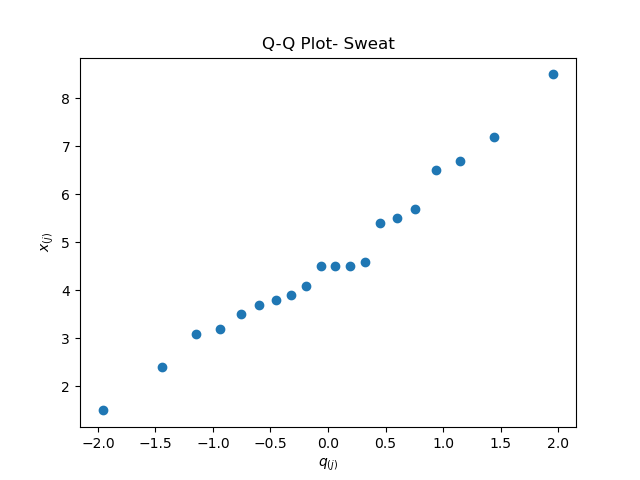
\includegraphics[scale=0.325]{./python/chapter-5/Question-5-4-QQ-Sweat.png} &
            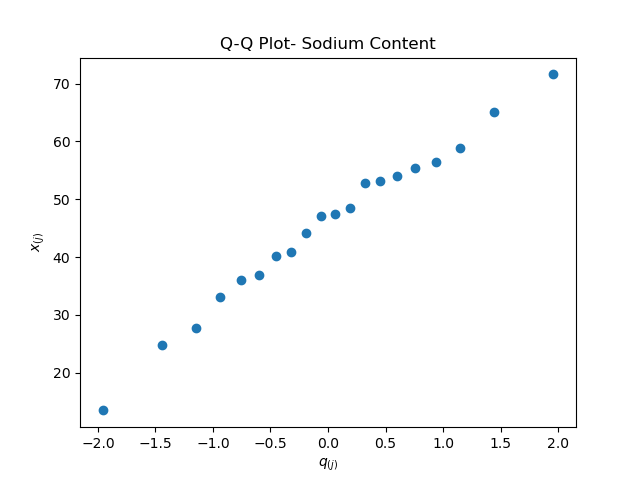
\includegraphics[scale=0.325]{./python/chapter-5/Question-5-4-QQ-Sodium.png} \\
            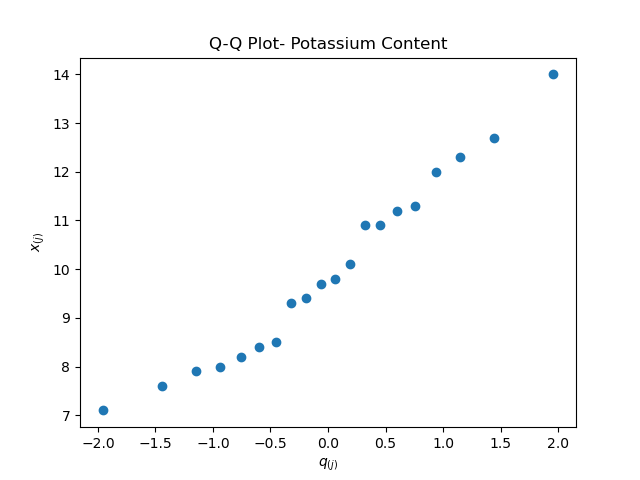
\includegraphics[scale=0.325]{./python/chapter-5/Question-5-4-QQ-Potassium.png}
        \end{tabular}
    \end{figure}

    \begin{figure}[H]
        \centering
        \begin{tabular}{cc}
            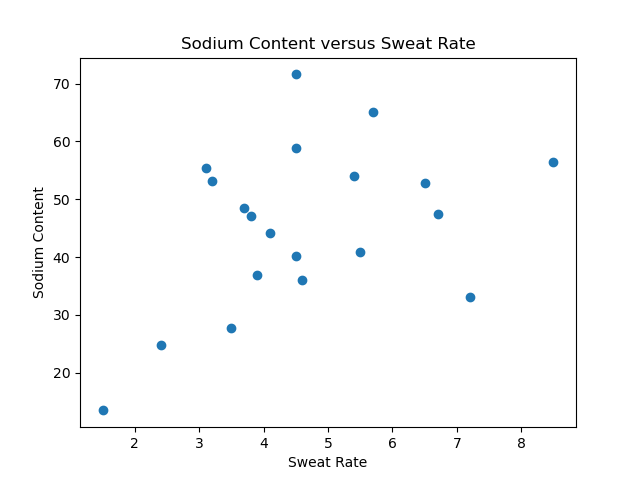
\includegraphics[scale=0.325]{./python/chapter-5/Question-5-4-Sweat-vs-Sodium.png} &
            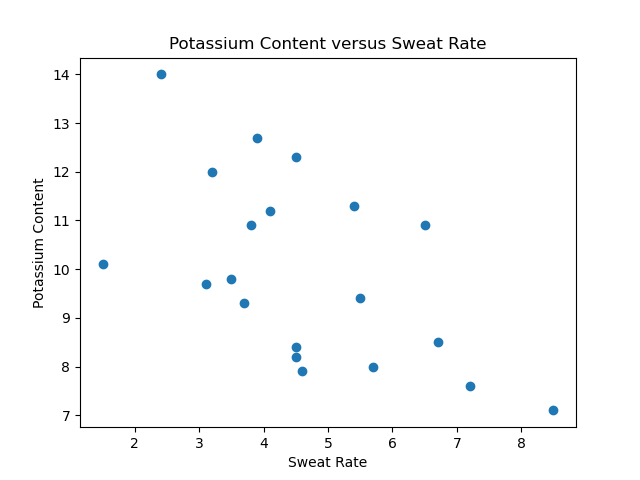
\includegraphics[scale=0.325]{./python/chapter-5/Question-5-4-Sweat-vs-Potassium.png} \\
            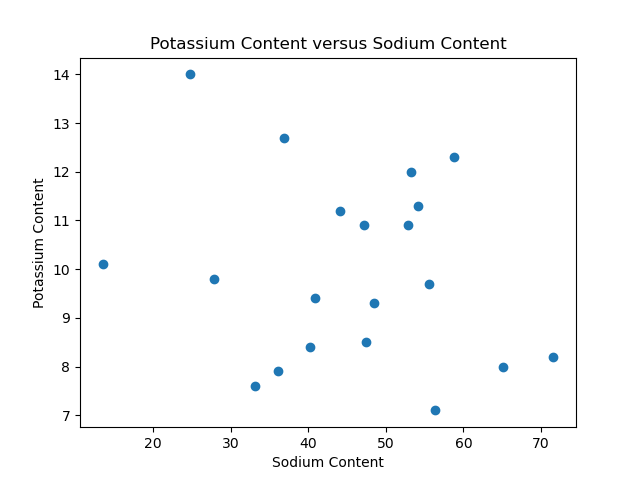
\includegraphics[scale=0.325]{./python/chapter-5/Question-5-4-Sodium-vs-Potassium.png}
        \end{tabular}
    \end{figure}

\end{enumerate}